\documentclass[11pt,fleqn]{article}
\usepackage[letterpaper,margin=0.92in]{geometry}
\usepackage{fontspec}
\usepackage{xeCJK}
\setmainfont{TeXGyrePagella}
\setsansfont{TeXGyreHeros}
\setmonofont{Noto Sans Mono CJK SC}
\setCJKmainfont{Noto Serif CJK SC}
\setCJKmonofont{Noto Sans Mono CJK SC}
\usepackage{eulervm}
\usepackage{microtype}
\usepackage{amsmath,amssymb,mathtools,amsthm}
\usepackage{xcolor}
\usepackage{hyperref}
\usepackage{graphicx}
\usepackage{enumitem}
\usepackage{booktabs}
\usepackage{array,tabularx}
\usepackage{listings}
\usepackage{fancyvrb}
\usepackage{fancyhdr}
\usepackage{tikz}
\usepackage{caption}
\captionsetup{font=small,labelfont=bf,labelsep=period}
\hypersetup{colorlinks=true,linkcolor=black,urlcolor=blue!55!black,citecolor=black}
\setlength{\parindent}{1.2em}
\setlength{\parskip}{0pt}
\setlength{\mathindent}{1.7em}
\setlist{nosep,leftmargin=1.6em}
\setlength{\headheight}{14pt}
\pagestyle{fancy}
\fancyhf{}
\fancyhead[L]{\small Ternatrees and A120590}
\fancyhead[R]{\small Bradley Klee}
\fancyfoot[C]{\thepage}
\renewcommand{\headrulewidth}{0.25pt}
\renewcommand{\footrulewidth}{0pt}

\theoremstyle{plain}
\newtheorem*{theorem}{Theorem}

\definecolor{codegray}{RGB}{95,95,95}
\definecolor{codebg}{RGB}{250,250,250}
\lstdefinestyle{pycode}{
  language=Python,
  basicstyle=\ttfamily\fontsize{7.25}{8.25}\selectfont,
  keywordstyle=\bfseries,
  commentstyle=\color{codegray},
  stringstyle=\itshape,
  showstringspaces=false,
  breaklines=true,
  breakatwhitespace=false,
  columns=fullflexible,
  keepspaces=true,
  frame=tb,
  framerule=0.3pt,
  rulecolor=\color{black!45},
  backgroundcolor=\color{codebg},
  numbers=left,
  numberstyle=\tiny\color{codegray},
  numbersep=5pt,
  xleftmargin=2.1em,
  framexleftmargin=1.8em,
  aboveskip=5pt,
  belowskip=4pt
}

\tikzset{
  ternroot/.style={circle,draw=black,fill=white,inner sep=2.0pt,line width=0.55pt},
  ternleaf/.style={circle,draw=black,fill=black,inner sep=2.0pt,line width=0.55pt},
  ternempty/.style={circle,draw=black,fill=white,inner sep=1.55pt,line width=0.55pt},
  ternedge/.style={draw=black,line width=0.55pt}
}

\newcommand{\poly}[1]{\langle #1\rangle}
\newcommand{\dd}{\,d}

\title{\vspace{-2.1em}\textbf{Ternatrees and OEIS A120590}\\[0.3em]
\large Integral, recurrence, and differential descriptions of an ordered tree class}
\author{Bradley Klee, \quad Harm.On.ica S-O-L 5.6 \textnormal{(OpenAI)}}
\date{}

\raggedbottom
\begin{document}
\maketitle
\thispagestyle{empty}

\begin{abstract}
The sequence $a(n)$ counts rooted ordered ternatrees with $n$ true leaves and
no unary branching.  Counting trees by their numbers of two-child and
three-child vertices gives a finite sum and a contour-integral formula for
each coefficient.  Summing these integrals gives an integral definition of
the ordinary generating function $A(x)$.  The local inverse of
$\rho(u)=u-3u^2-u^3$ then yields the algebraic equation for $A(x)$.  Two exact
reductions of the same integral family are compared: a shift reduction in $n$
gives a second-order recurrence, while a parameter reduction in $x$ gives a
differential equation.  Their $6\times6$ reduction matrices satisfy
$G_x=G-x\operatorname{diag}(I_3,0)$.
\end{abstract}

\begin{theorem}
Let $a(n)$ be the number of rooted ordered ternatrees with $n$ true leaves and
no unary branching, and let
\[
A(x)=\sum_{n\ge0}a(n)x^n.
\]
Then:
\begin{enumerate}[label=(\arabic*),leftmargin=2.2em,itemsep=0.55em,topsep=0.35em]
\item Put $D(u)=1-3u-u^2$ and $\rho(u)=uD(u)$.  For a sufficiently small
positively oriented circle $\gamma$ about the origin,
\[
a(0)=1,\qquad
 a(n)=\frac{1}{2\pi i\,n}\oint_\gamma\frac{\dd u}{\rho(u)^n}
     =\frac1n[u^{n-1}]D(u)^{-n}\qquad(n\ge1).
\]
For $|x|$ sufficiently small, with the logarithm chosen continuously from
$x=0$,
\[
A(x)=1-\frac{1}{2\pi i}\oint_\gamma
\log\!\left(1-\frac{x}{\rho(u)}\right)\dd u.
\]
\item The integral definition implies
\[
4A(x)=3+x+A(x)^3,\qquad A(0)=1.
\]
\item For $n\ge1$,
\begin{center}
\small
$-3(3n-1)(3n+1)a(n)-81(n+1)(2n+1)a(n+1)+13(n+1)(n+2)a(n+2)=0.$
\end{center}
\item The generating function satisfies
\[
(27x^2+162x-13)A''(x)+27(x+3)A'(x)-3A(x)=0.
\]
\end{enumerate}
The initial values are
\[
1,1,3,19,150,1326,12558,124590,\ldots.
\]
\end{theorem}

\clearpage
\section{From ternatrees to the integral form}

A ternatree is a rooted ordered tree in which every internal vertex has three
ordered child positions.  A position may be empty, may contain a true leaf, or
may contain another internal vertex.  Every internal vertex has either two or
three occupied positions; unary branching is excluded.

\begin{figure}[h]
\centering
\begin{minipage}[t]{0.22\textwidth}\centering
\begin{tikzpicture}[x=1cm,y=1cm,scale=1.0]
  \node[ternleaf] at (0,0.7) {};
\end{tikzpicture}
\par\smallskip\(1\)
\end{minipage}\hfill
\begin{minipage}[t]{0.22\textwidth}\centering
\begin{tikzpicture}[x=1cm,y=1cm,scale=1.0]
  \node[ternroot] (r) at (0,1.15) {};
  \node[ternleaf] (a) at (-0.62,0) {};
  \node[ternleaf] (b) at (0,0) {};
  \node[ternempty] (c) at (0.62,0) {};
  \draw[ternedge] (r)--(a) (r)--(b) (r)--(c);
\end{tikzpicture}
\par\smallskip\(\{1,1,0\}\)
\end{minipage}\hfill
\begin{minipage}[t]{0.22\textwidth}\centering
\begin{tikzpicture}[x=1cm,y=1cm,scale=1.0]
  \node[ternroot] (r) at (0,1.15) {};
  \node[ternleaf] (a) at (-0.62,0) {};
  \node[ternleaf] (b) at (0,0) {};
  \node[ternleaf] (c) at (0.62,0) {};
  \draw[ternedge] (r)--(a) (r)--(b) (r)--(c);
\end{tikzpicture}
\par\smallskip\(\{1,1,1\}\)
\end{minipage}\hfill
\begin{minipage}[t]{0.28\textwidth}\centering
\begin{tikzpicture}[x=1cm,y=1cm,scale=1.0]
  \node[ternroot] (r) at (0,2.0) {};
  \node[ternroot] (a) at (-0.72,1.03) {};
  \node[ternleaf] (b) at (0,1.03) {};
  \node[ternempty] (c) at (0.72,1.03) {};
  \node[ternleaf] (aa) at (-1.15,0) {};
  \node[ternleaf] (ab) at (-0.72,0) {};
  \node[ternempty] (ac) at (-0.29,0) {};
  \draw[ternedge] (r)--(a) (r)--(b) (r)--(c);
  \draw[ternedge] (a)--(aa) (a)--(ab) (a)--(ac);
\end{tikzpicture}
\par\smallskip\(\{\{1,1,0\},1,0\}\)
\end{minipage}
\caption{Representative ternatrees.  Filled endpoints are true leaves, open
endpoints are empty child positions, and horizontal order records the three
ordered slots.}
\end{figure}

Fix a ternatree with $n$ true leaves, $i$ internal vertices having two occupied
positions, and $j$ internal vertices having three occupied positions.  Counting
edges in two ways gives
\[
n-1=i+2j.
\]
The tree has $m=n+i+j$ vertices.  In preorder, write $-1$ for a leaf, $+1$ for
a two-child vertex, and $+2$ for a three-child vertex.  The resulting word has
total sum $-1$.  By the cycle lemma, exactly one of its $m$ cyclic rotations
has the partial-sum condition of a rooted ordered tree.  There are three choices
for the empty position at every two-child vertex.  Hence the number of trees
with this profile is
\[
\frac{3^i}{m}\binom{m}{n,i,j}.
\]
Putting $j=k$, $i=n-1-2k$, and $m=2n-1-k$ yields
\[
a(n)=\sum_{k=0}^{\lfloor(n-1)/2\rfloor}
3^{n-1-2k}\frac{(2n-2-k)!}{n!\,(n-1-2k)!\,k!}\qquad(n\ge1).
\]
Equivalently,
\[
a(n)=\frac1n\sum_{k=0}^{\lfloor(n-1)/2\rfloor}
3^{n-1-2k}
\binom{2n-2-k}{n-1}
\binom{n-1-k}{k}.
\]
Expanding $(1-3u-u^2)^{-n}$ gives precisely this sum, so with
\[
D(u)=1-3u-u^2,
\]
one obtains
\[
a(n)=\frac1n[u^{n-1}]D(u)^{-n}.
\]
Cauchy's coefficient formula gives the integral form:
\[
\rho(u)=uD(u)=u-3u^2-u^3,\qquad
a(n)=\frac{1}{2\pi i\,n}\oint_\gamma
\frac{\dd u}{u^nD(u)^n}
=\frac{1}{2\pi i\,n}\oint_\gamma\frac{\dd u}{\rho(u)^n}.
\]

The coefficient integrals may now be summed before any algebraic equation is
introduced.  Choose $\gamma$ so that $|x|<|\rho(u)|$ on the contour.  Then
uniform convergence permits termwise summation:
\[
\begin{aligned}
A(x)
&=1+\sum_{n\ge1}\frac{x^n}{2\pi i\,n}
  \oint_\gamma\frac{\dd u}{\rho(u)^n}\\
&=1+\frac{1}{2\pi i}\oint_\gamma
  \sum_{n\ge1}\frac1n\left(\frac{x}{\rho(u)}\right)^n\dd u\\
&=1-\frac{1}{2\pi i}\oint_\gamma
  \log\!\left(1-\frac{x}{\rho(u)}\right)\dd u.
\end{aligned}
\]
This is the integral definition of the ordinary generating function near the
origin.

The algebraic equation follows from this integral definition.  Differentiating
under the integral sign gives
\[
A'(x)=\frac{1}{2\pi i}\oint_\gamma
\frac{\dd u}{\rho(u)-x}.
\]
Since $\rho(0)=0$ and $\rho'(0)=1$, there is a unique analytic function
$T(x)$ near the origin satisfying $T(0)=0$ and $\rho(T(x))=x$.  For small
$x$, this is the only zero of $\rho(u)-x$ inside $\gamma$.  Factor
\[
\rho(u)-x=(u-T(x))Q(x,u),
\qquad Q(x,T(x))=\rho'(T(x)).
\]
Cauchy's integral formula gives
\[
A'(x)=\frac{1}{Q(x,T(x))}
      =\frac{1}{\rho'(T(x))}
      =T'(x).
\]
Because $A(0)=1$ and $T(0)=0$, one has $A(x)=1+T(x)$.  Substitution into
$x=\rho(T)$ therefore gives
\[
x=(A-1)-3(A-1)^2-(A-1)^3,
\]
or equivalently
\[
4A=3+x+A^3.
\]

\clearpage
\section{Shift reduction and the recurrence}

For $n\ge1$, write
\[
H_n(u)=\frac1{n\rho(u)^n},\qquad
 a(n)=\frac{1}{2\pi i}\oint_\gamma H_n(u)\dd u.
\]
For $w=(w_0,w_1,w_2)^T$, put $\poly{w}=w_0+w_1u+w_2u^2$.  The
fixed reduction operators are
\[
U=\frac1{13}
\begin{pmatrix}
153&24&3\\72&9&6\\0&0&0
\end{pmatrix},\qquad
V=\frac1{13}
\begin{pmatrix}
-13&0&0\\75&11&3\\24&3&2
\end{pmatrix},\qquad
J=\begin{pmatrix}0&1&0\\0&0&2\\0&0&0\end{pmatrix}.
\]
They satisfy $\rho\poly{Uw}-\rho'\poly{Vw}=\poly{w}$, while
$\poly{Jw}=d(\poly{w})/du$.  Hence, for $m\ge1$,
\[
\frac{\poly{w}}{\rho^{m+1}}
=
\frac{\poly{(U-JV/m)w}}{\rho^m}
+\frac{d}{du}\left(\frac{\poly{Vw}}{m\rho^m}\right).
\]
The integral of the last term around $\gamma$ is zero, so each application
removes one power of $\rho$ and leaves a vector in the same
three-dimensional numerator space.

With $e=(1,0,0)^T$, define
\[
c_0=e,\qquad
c_1=\frac{n}{n+1}\operatorname{Lower}(e,n),\qquad
c_2=\frac{n}{n+2}\operatorname{Lower}
   (\operatorname{Lower}(e,n+1),n).
\]
Their third components vanish.  The first two components form a $2\times3$
remainder matrix $X(n)$ whose one-dimensional kernel is generated by
\[
P_0(n)=-3(3n-1)(3n+1),\qquad
P_1(n)=-81(n+1)(2n+1),\qquad
P_2(n)=13(n+1)(n+2).
\]
The kernel relation lifts to the exact identity
\[
P_0H_n+P_1H_{n+1}+P_2H_{n+2}
=\frac{d}{du}\bigl(R(n,u)H_n(u)\bigr),
\]
where
\[
R(n,u)=
\frac{-9nu^4-36nu^3+6nu^2+84nu-13n-3u^4-12u^3-6u^2+3u}{\rho(u)}.
\]
Integrating around $\gamma$ gives
\[
P_0(n)a(n)+P_1(n)a(n+1)+P_2(n)a(n+2)=0.
\]

\clearpage
\section{Direct reduction in the generating variable}

Both reductions arise from the coefficient map
\[
M_q(a,b)=q(u)a(u)-\rho'(u)b(u),
\]
where $a(u)$ and $b(u)$ have degree less than three.  In the basis
$1,u,\ldots,u^5$, the specialization $q=\rho$ is represented by
\[
G=
\begin{pmatrix}
0&0&0&-1&0&0\\
1&0&0&6&-1&0\\
-3&1&0&3&6&-1\\
-1&-3&1&0&3&6\\
0&-1&-3&0&0&3\\
0&0&-1&0&0&0
\end{pmatrix},
\qquad \det G=-13.
\]
Let $E=\binom{I_3}{0}$.  The relation
\[
G^{-1}E=\binom{U}{V}
\]
produces exactly the operators used in Section 2.  Thus $G$ is the fixed
coefficient map for the shift reduction and the natural starting point for the
direct comparison.

Differentiating the generating-function integral obtained in Section 1 gives
\[
A'(x)=\frac{1}{2\pi i}\oint_\gamma F(x,u)\dd u,
\qquad
F(x,u)=\frac1{g(x,u)},
\qquad
g(x,u)=\rho(u)-x.
\]
Replacing $q=\rho$ by $q=g$ changes only the upper-left block of the
coefficient map:
\[
G_x=
\begin{pmatrix}
-x&0&0&-1&0&0\\
1&-x&0&6&-1&0\\
-3&1&-x&3&6&-1\\
-1&-3&1&0&3&6\\
0&-1&-3&0&0&3\\
0&0&-1&0&0&0
\end{pmatrix}.
\]
Consequently,
\[
G_x=G-x\begin{pmatrix}I_3&0\\0&0\end{pmatrix}
    =G-xEE^T,
\qquad
\det G_x=27x^2+162x-13,
\qquad
G_x^{-1}E=\binom{U_x}{V_x}.
\]
The same pole-lowering identity holds with $\rho$ replaced by $g$ and
$(U,V)$ replaced by $(U_x,V_x)$.  Reducing $F$, $\partial_xF$, and
$\partial_x^2F$ gives three columns in the same two-dimensional remainder
space.  Their kernel is generated by
\[
\begin{pmatrix}
24\\81x+243\\27x^2+162x-13
\end{pmatrix}.
\]
The corresponding exact identity is
\[
24F+(81x+243)\partial_xF+(27x^2+162x-13)\partial_x^2F
=
\frac{d}{du}\left(\frac{N(x,u)}{g(x,u)^2}\right),
\]
where
\[
N(x,u)=12u^4+48u^3+3ux-87u+3x+13.
\]
After integration around $\gamma$,
\[
(27x^2+162x-13)A'''(x)+(81x+243)A''(x)+24A'(x)=0.
\]
This is the derivative of
\[
(27x^2+162x-13)A''(x)+27(x+3)A'(x)-3A(x)=C.
\]
The initial values $A(0)=1$, $A'(0)=1$, and $A''(0)=6$ give $C=0$.

\section{Comparison of the two reductions}

The two calculations are instances of the same exact reduction.  They differ
only in the family placed under the contour integral and in the coefficient
field of the inverse matrix.

\begin{center}
\renewcommand{\arraystretch}{1.22}
\begin{tabularx}{\textwidth}{>{\raggedright\arraybackslash}p{0.20\textwidth}
                              >{\raggedright\arraybackslash}X
                              >{\raggedright\arraybackslash}X}
\toprule
& \textbf{Shift in $n$} & \textbf{Derivative in $x$}\\
\midrule
Integral family
& $H_{n+r}(u)=1/((n+r)\rho(u)^{n+r})$
& $\partial_x^rF(x,u)=r!/g(x,u)^{r+1}$\\
Denominator
& $\rho(u)$
& $g(x,u)=\rho(u)-x$\\
Coefficient map
& $G$
& $G_x=G-xEE^T$\\
Inverse blocks
& $U,V$ over $\mathbb Q$
& $U_x,V_x$ over $\mathbb Q(x)$\\
Reduced columns
& $H_n,H_{n+1},H_{n+2}$
& $F,\partial_xF,\partial_x^2F$\\
Kernel
& $(P_0(n),P_1(n),P_2(n))^T$
& $(24,81x+243,\det G_x)^T$\\
Integral consequence
& recurrence for $a(n)$
& differential equation for $A(x)$\\
\bottomrule
\end{tabularx}
\end{center}

At $x=0$, the direct matrix specializes to the shift matrix:
\[
G_x\big|_{x=0}=G,
\qquad
\det G_x\big|_{x=0}=\det G=-13.
\]
The determinant plays the same structural role in both calculations.  Its
constant value supplies the denominator $13$ in $U$ and $V$ and the leading
coefficient $13(n+1)(n+2)$ of the recurrence.  Its polynomial deformation is
the leading coefficient of the differential equation.

The differential equation reproduces the recurrence without any further
symbolic reduction.  Multiplying it by $-1$ gives
\[
(13-162x-27x^2)A''-27(x+3)A'+3A=0.
\]
The coefficient of $x^n$ is
\[
(-27n^2+3)a(n)+(-162n^2-243n-81)a(n+1)
 +(13n^2+39n+26)a(n+2),
\]
which is exactly
\[
P_0(n)a(n)+P_1(n)a(n+1)+P_2(n)a(n+2).
\]
Thus the two kernels encode the same relation in the discrete and generating
variables.

The shared mechanism may be summarized by writing
\[
M_q(a,b)=q(u)a(u)-\rho'(u)b(u),
\qquad M_\rho=G,\qquad M_g=G_x.
\]
If $M_q^{-1}E=\binom{U_q}{V_q}$, then both calculations use
\[
\frac{\poly{w}}{q^{m+1}}
=
\frac{\poly{(U_q-JV_q/m)w}}{q^m}
+\frac{d}{du}\left(\frac{\poly{V_qw}}{mq^m}\right).
\]
The inverses display the parallel leading factors directly:
\[
G^{-1}=\frac{\operatorname{adj}(G)}{-13},
\qquad
G_x^{-1}=\frac{\operatorname{adj}(G_x)}{27x^2+162x-13}.
\]
In each route, three reduced columns lie in a two-dimensional space:
\[
\begin{array}{rcl}
(H_n,H_{n+1},H_{n+2})&\longmapsto&X(n)
   \longmapsto \ker X(n)=\langle P(n)\rangle,\\[0.35em]
(F,\partial_xF,\partial_x^2F)&\longmapsto&X_x(x)
   \longmapsto \ker X_x(x)=\langle C(x)\rangle.
\end{array}
\]

\clearpage
\section{Reference pseudocode}

The following specification implements the shift reduction.  It constructs the
remainder matrix, extracts its primitive kernel vector, generates the sequence,
and converts the recurrence into the differential equation.
\begin{center}
\begin{minipage}{0.96\textwidth}
\VerbatimInput[fontsize=\fontsize{7.4}{8.4}\selectfont,frame=lines]
{ternatree_one_page_crank_academic.txt}
\end{minipage}
\end{center}

\clearpage
\section{Pseudocode operations and exact realization}
\begin{figure}[h]
\centering
\begin{minipage}[t]{0.485\textwidth}
\centering
\textbf{(a) Pseudocode}\par\smallskip
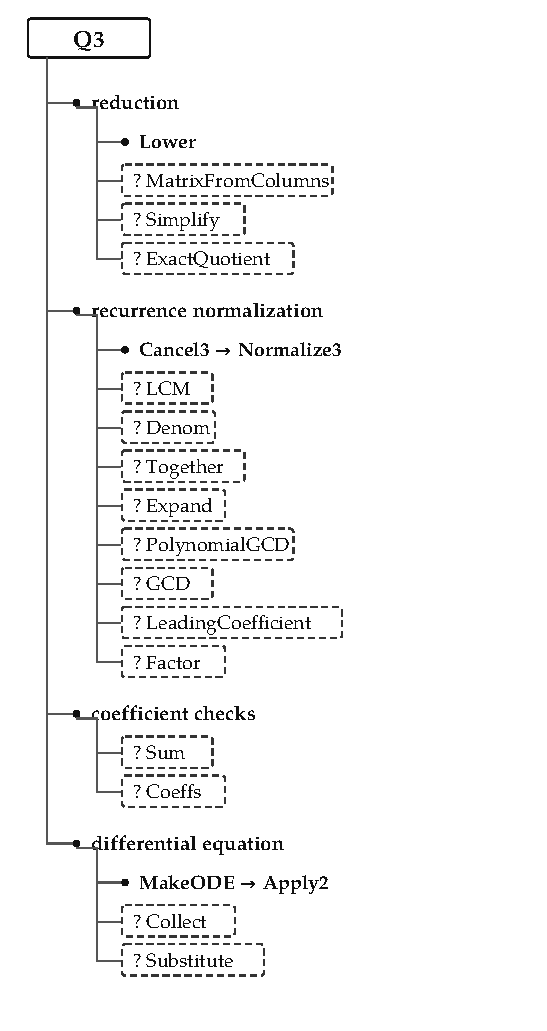
\includegraphics[width=\linewidth,height=0.75\textheight,keepaspectratio]
{../graphs/ternatree_pseudocode_mysteries.pdf}
\end{minipage}\hfill
\begin{minipage}[t]{0.485\textwidth}
\centering
\textbf{(b) SymPy implementation}\par\smallskip
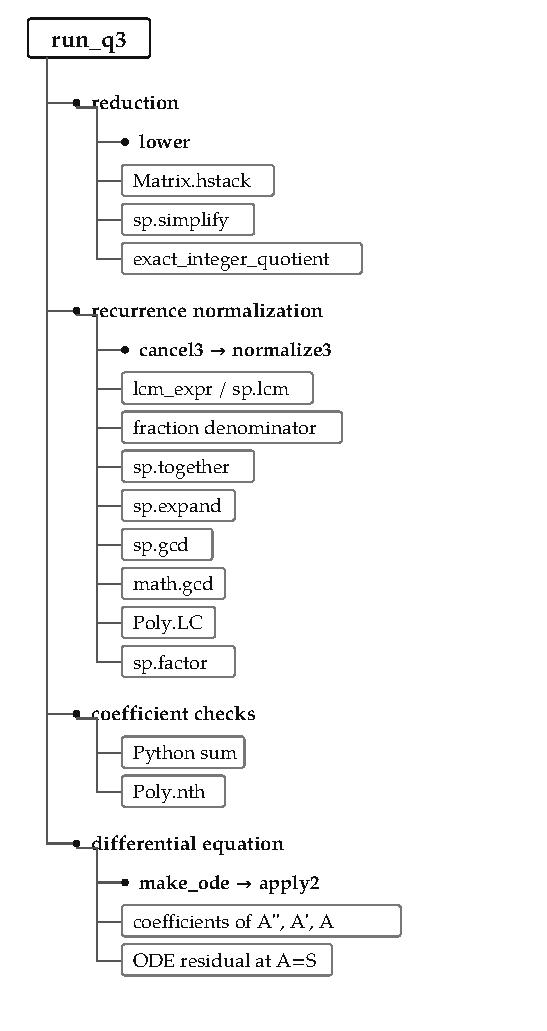
\includegraphics[width=\linewidth,height=0.75\textheight,keepaspectratio]
{../graphs/ternatree_sympy_resolutions.pdf}
\end{minipage}
\caption{The local routines and their algebraic dependencies.  Dashed leaves
are operations used but not defined in the pseudocode; the corresponding rows
on the right identify their exact realization.}
\end{figure}

\clearpage
\section{Relations among the formulas}

The geometric count, integral definition, recurrence, algebraic equation, and
differential equation determine the same series.  Their relations are
\[
\begin{array}{c}
\text{ternatree profiles}
\longrightarrow
\displaystyle a(n)=\frac{1}{2\pi i\,n}\oint_\gamma\frac{\dd u}{\rho(u)^n}
\longrightarrow
\displaystyle A(x)=1-\frac{1}{2\pi i}\oint_\gamma
\log\!\left(1-\frac{x}{\rho(u)}\right)\dd u,\\[1.1em]
\text{local inverse }\rho(T)=x
\longrightarrow
A=1+T
\longrightarrow
4A=3+x+A^3,\\[1.1em]
\text{shift reduction of the coefficient integral}
\longrightarrow
\text{recurrence},\\[0.6em]
\text{parameter reduction of the generating-function integral}
\longrightarrow
\text{differential equation}.
\end{array}
\]
The recurrence and differential equation correspond coefficient by
coefficient, and either one generates the terms of A120590 from the stated
initial values.

\appendix
\section{Exact SymPy implementation}

This implementation merges one-shot code produced independently by Kimi (Moonshot AI) and Claude (Anthropic AI), both working from the pseudocode presented in Section 5.

\subsection{Arithmetic and one-step lowering}
The functions below define exact least common multiples and the map
$w\mapsto (U-JV/m)w$.
\par\medskip\noindent
\begin{minipage}[t]{\textwidth}
\lstinputlisting[style=pycode,firstline=1,lastline=24,firstnumber=1]
{../../ternatree_q3.py}
\end{minipage}

\clearpage
\subsection{Primitive recurrence normalization}
This function clears rational denominators, removes common polynomial and
integer factors, and fixes the sign of the recurrence vector.
\par\medskip\noindent
\begin{minipage}[t]{\textwidth}
\lstinputlisting[style=pycode,firstline=26,lastline=58,firstnumber=26]
{../../ternatree_q3.py}
\end{minipage}

\clearpage
\subsection{Kernel vector and recurrence-to-ODE map}
The $2\times3$ minors form the kernel vector.  The remaining functions convert
quadratic recurrence coefficients into the coefficients of $A''$, $A'$, and
$A$.
\par\medskip\noindent
\begin{minipage}[t]{\textwidth}
\lstinputlisting[style=pycode,firstline=61,lastline=99,firstnumber=61]
{../../ternatree_q3.py}
\end{minipage}

\clearpage
\subsection{Term generation and exact checks}
The driver enters $U,V,J$, constructs $X$, derives the recurrence, generates
terms, and checks the algebraic and differential equations.
\par\medskip\noindent
\begin{minipage}[t]{\textwidth}
\lstinputlisting[style=pycode,basicstyle=\ttfamily\fontsize{6.65}{7.45}\selectfont,
 firstline=102,lastline=167,firstnumber=102]
{../../ternatree_q3.py}
\end{minipage}

\end{document}
